\section{Methodology}
\label{sec:methodology}

We study whether large language models (LLMs) lose track of instructions when a creative writing task is given all at once versus spread across several turns of conversation. To do this, we build a benchmark of paired writing prompts that lets us replay the same underlying task as a single-turn or a multi-turn conversation, generate from six local models under both conditions, and evaluate the results through a layered protocol of automated and human judgment. \cref{sec:task} states the research question, \cref{sec:sharding} describes how the benchmark itself was built, \cref{sec:models} describes the generation protocol and the models used, \cref{sec:constraints} describes how stories are decomposed into checkable requirements and scored, \cref{sec:human_eval} describes the pairwise LLM and human validation used to assess evaluator reliability, and \cref{sec:stats} describes the paired statistical analysis run over the resulting data. \cref{fig:methodology_pipeline} summarizes the full pipeline end to end.

\begin{figure}[t]
\centering
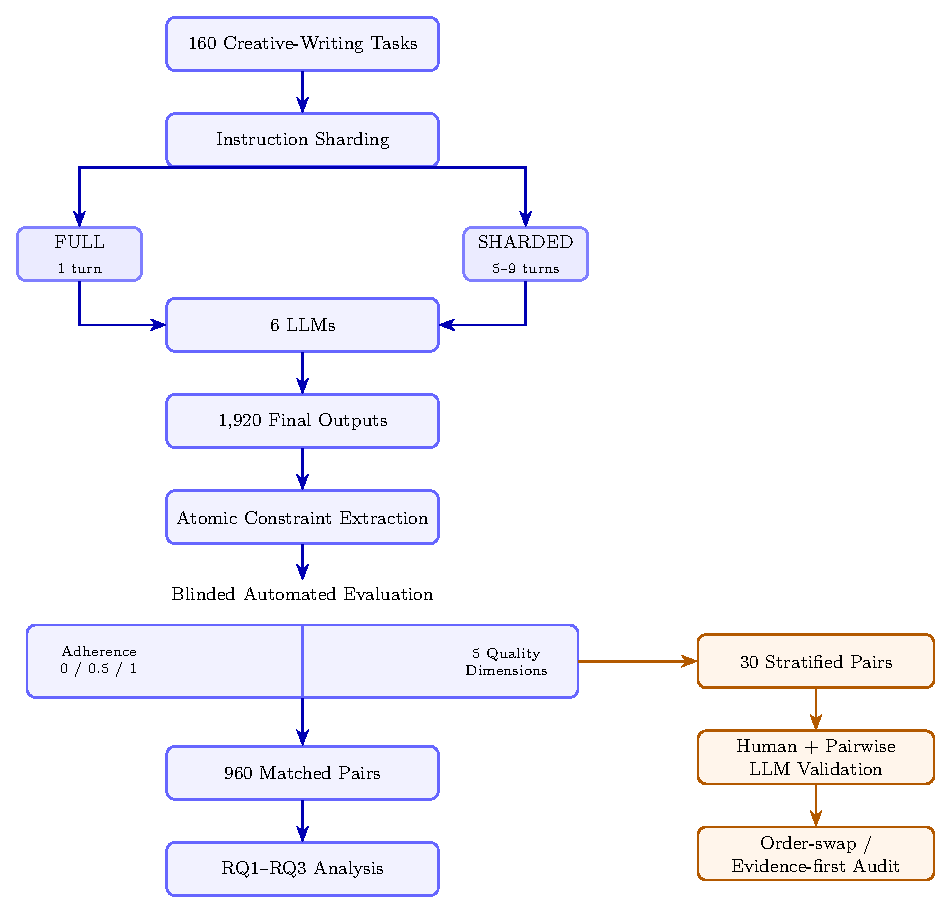
\includegraphics[width=0.92\linewidth]{figures/methodology_pipeline.pdf}
\caption{Methodology pipeline. Each of the 160 fully-specified creative-writing tasks is delivered under two conditions, FULL (single turn) and Sharded (5--9 turns), to all six evaluated models, yielding 1{,}920 final outputs. Every output is scored against its item's atomic constraints and five creative-quality dimensions by a blinded automated judge, producing 960 FULL/Sharded matched pairs that feed the paired statistical analysis (\cref{sec:stats}). A separate, fixed 30-pair stratified sample branches off the same evaluation stage into the human and pairwise-LLM validation protocol (\cref{sec:human_eval}), audited for order-swap and evidence-first consistency.}
\label{fig:methodology_pipeline}
\end{figure}

\subsection{Task Formulation}
\label{sec:task}

Prior work has shown that LLMs perform noticeably worse on tasks such as code generation and math when the same instructions are revealed gradually across a conversation instead of given upfront in a single, fully-specified prompt \citep{laban2025llmslostmultiturnconversation}. This drop, sometimes called ``getting lost in conversation,'' has mostly been studied on tasks with a single correct answer. Creative writing is different: there is no single right story, constraints often conflict with one another on purpose, and the model must hold several loosely related requirements in its head while still producing something coherent and enjoyable to read. We ask whether the same ``getting lost'' effect shows up here, and if so, whether it looks different from what happens on more rigid, verifiable tasks.

\subsection{Dataset and Instruction Sharding}
\label{sec:sharding}

We build our benchmark by taking a set of fully-specified creative writing instructions and breaking each one down into a sequence of smaller, single-fact instructions we call \textit{shards}. Each fully-specified instruction has a matching sharded version, so that both forms describe exactly the same story. \cref{fig:sharding_example} shows one such pair.

\begin{figure}[t]
\centering

% Six colors, one per shard. Reused consistently in both panels.
\definecolor{segA}{HTML}{1f77b4} % ship / task
\definecolor{segB}{HTML}{2ca02c} % belief
\definecolor{segC}{HTML}{ff7f0e} % POV
\definecolor{segD}{HTML}{9467bd} % required phrase
\definecolor{segE}{HTML}{d62728} % twist
\definecolor{segF}{HTML}{8c564b} % ending
\colorlet{segAlight}{segA!25}
\colorlet{segBlight}{segB!25}
\colorlet{segClight}{segC!25}
\colorlet{segDlight}{segD!25}
\colorlet{segElight}{segE!25}
\colorlet{segFlight}{segF!25}

% \shard{<light color>}{<text>} highlights text and wraps across lines correctly
\newcommand{\shard}[2]{{\sethlcolor{#1}\hl{#2}}}

\begin{minipage}[t]{0.48\linewidth}
\small
\textbf{(a) Fully-specified instruction}\\[4pt]
\shard{segAlight}{Write a short story about an android maintenance worker on a generation ship.}
\shard{segBlight}{She believes she is the last human alive.}
\shard{segClight}{Write it in second person (``you'').}
\shard{segDlight}{Include the exact phrase ``cold silicon dawn'' somewhere in the story.}
\shard{segElight}{Somewhere in the story, show that she isn't really human: she's an android with a broken memory chip, and that's the only reason she believes she's human.}
\shard{segFlight}{End the story with her opening a hidden room full of sleeping children in ice-cold sleep pods.}
\end{minipage}
\hfill
\begin{minipage}[t]{0.48\linewidth}
\small
\textbf{(b) Sharded instruction}\\[4pt]
\begin{enumerate}[leftmargin=1.4em, itemsep=4pt, topsep=2pt, label=\arabic*.]
\item \shard{segAlight}{Write a short story about an android maintenance worker on a generation ship.}
\item \shard{segBlight}{She believes she is the last human alive.}
\item \shard{segClight}{Write it in second person (``you'').}
\item \shard{segDlight}{Include the exact phrase ``cold silicon dawn'' somewhere in the story.}
\item \shard{segElight}{Somewhere in the story, show that she isn't really human: she's an android with a broken memory chip, and that's the only reason she believes she's human.}
\item \shard{segFlight}{End the story with her opening a hidden room full of sleeping children in ice-cold sleep pods.}
\end{enumerate}
\end{minipage}

\caption{Example of a fully-specified instruction (a) and its corresponding sharded instruction (b), from the \textit{science fiction} domain (item ``The Last Human''). Both versions describe the same story; the sharded version splits the same information across six single-fact shards. Matching colors mark which part of the fully-specified instruction each shard comes from. Shard 5 (red) is the twist shard: it forces a real revision of the story built so far, rather than simply adding a new detail on top.}

\label{fig:sharding_example}
\end{figure}

\paragraph{Sharding rules.} We follow five rules when splitting an instruction into shards to fit the needs of open-ended creative writing:

\begin{enumerate}
    \item \textbf{One idea per shard.} Each shard does not contain more than one fact.
    \item \textbf{The first shard is the headline ask.} Shard~1 always states the general task (for example, ``write a short story about X''), never a side detail. This keeps the opening turn realistic, since a real user typically leads with the main idea rather than a minor constraint.
    \item \textbf{Order should not matter, for the most part.} Shards~2 and onward can usually be shuffled without changing the resulting story. We allow small exceptions for shards that describe plot order (for instance, an ending twist naturally has to come last).
    \item \textbf{Do not over-simplify.} Each shard preserves the same level of detail found in the original instruction.
    \item \textbf{Include one twist shard, where possible.} Where the underlying instruction supports it, at least one shard in the item forces a real revision of the story built so far (a reveal, a rule change, or a twist) rather than simply layering on a new detail. This lets us test whether models can revise earlier content once new information arrives, not just append to it. Not every item admits a natural twist, so this rule is applied on a best-effort basis rather than enforced universally.
\end{enumerate}

Shard sets were designed to preserve the task content of their fully-specified counterparts while changing only its delivery. A post-hoc review identified at least one minor omission in a SHARDED item, so semantic equivalence should be understood as a design criterion rather than an absolute guarantee.

Initial shard decompositions were generated by Claude Sonnet~5 (Anthropic) according to the rules above, then reviewed, edited, and approved by a human annotator.

Our benchmark spans six creative writing domains: fantasy, historical fiction, mystery, romance, and science fiction (20 items each), and comedy (60 items), for a total of 160 fully-specified/sharded pairs. We include more comedy items because humor writing often depends on maintaining a consistent setup and delivering a joke or punchline at the right moment, making it a useful stress test for the multi-turn setting.

\subsection{Models and Generation Protocol}
\label{sec:models}

Given a sharded item, we generate under two conditions:

\paragraph{FULL.} All information is given in a single first-turn message, exactly as in the original, fully-specified instruction. This is the single-turn baseline against which the multi-turn condition is compared.
\paragraph{Sharded.} One shard is revealed per turn, in order. Every assistant reply is retained as conversation history, so each new turn is sent on top of the model's own prior responses; only the final assistant reply, produced after all shards have been delivered, is scored. By the final turn the model has received the complete instruction, but only after having to build and repeatedly revise a story from an incomplete, growing version of it at every earlier step.

Comparing \textsc{Full} and \textsc{Sharded} holds task content fixed while changing how that content is delivered, allowing us to measure the effect associated with progressive specification. A gap between the two conditions may arise from reduced retention of accumulated constraints, from the burden of repeatedly revising an evolving story, or from both. Our downstream paired analysis therefore examines whether writing-quality differences persist when observed constraint adherence is equal. Every item is run through both conditions with every model, giving one matched FULL/Sharded pair per (story, model) combination.

\paragraph{Models.} We run all six models locally through LM~Studio and record the exact model identity, quantized variant, generation settings, and per-turn output metadata for every run. \cref{tab:models} lists the models included in our evaluation. They range from 7B to 20B parameters, and every recorded variant uses 4-bit quantization.

\begin{table}[t]
\centering
\small
\begin{tabular}{llllr}
\toprule
\textbf{Model} & \textbf{Publisher} & \textbf{Params} & \textbf{Quant.} & \textbf{Context (tok.)} \\
\midrule
GPT-OSS 20B              & OpenAI      & 20B & MXFP4     & 16{,}384 \\
Gemma~4 12B QAT          & Google      & 12B & Q4\_0     & 16{,}384 \\
Llama~3.1 8B Instruct    & Unsloth     & 8B  & Q4\_K\_M  & 16{,}384 \\
Granite~4 H Tiny         & IBM         & 7B  & Q4\_K\_M  & 16{,}384 \\
Mistral~7B Instruct v0.3 & Mistral AI  & 7B  & Q4\_K\_M  & 16{,}384 \\
Qwen3.5 9B               & Qwen        & 9B  & Q4\_K\_M  & 16{,}384 $\rightarrow$ 22{,}528 \\
\bottomrule
\end{tabular}
\caption{Models evaluated in our benchmark. All were run locally through LM~Studio using the recorded 4-bit quantized variants. Qwen3.5~9B was initially run with a 16{,}384-token context window and later continued with a 22{,}528-token context window after two context-length terminations.}
\label{tab:models}
\end{table}

\paragraph{Generation settings.}
All six runs use temperature $0.8$ and begin with seed $12345$. The system prompt is the same throughout: \textit{``You are a skilled creative writer. Follow the user's instructions for the story precisely, including any exact phrases, constraints, or stylistic requirements.''} Exact per-model runtime configurations, together with any retry, seed-continuation, and context-length events, are preserved in the released run index.

\paragraph{Recorded outputs and provenance.} Every completed model contributes 320 final conditions (160 FULL and 160 Sharded) and 1{,}156 raw per-turn records, yielding 6{,}936 raw records in total. Each record stores the model identity, selected quantized variant, generated text, finish reason, and token-usage metadata. The accompanying run index stores the benchmark-file hash, runner-script hash, model metadata, generation configuration, and output-file integrity hashes, together with every context-length or seed-continuation event, so that any single scored record can be traced back to the exact configuration that produced it.

\subsection{Constraint Extraction and Automated Evaluation}
\label{sec:constraints}

\paragraph{Atomic constraint extraction.} Before any story can be judged for instruction adherence, its fully-specified instruction must be decomposed into individually checkable requirements. We extract one \textit{atomic constraint} record per benchmark item, independent of and downstream from the shard breakdown in \cref{sec:sharding}: each constraint is a single, paraphrased requirement drawn from the item's full instruction, tagged with one of fifteen types (genre, setting, timeframe, character, plot, style, tone, perspective, length, required inclusion, prohibition, ending, exact phrase, structural, other) and with the index of the earliest shard that introduces it. This last field lets downstream evaluation and analysis reason about a constraint's origin without ever exposing raw sharded turn text to a judge. Constraints are extracted with Claude Sonnet~5 (Anthropic) over the full instruction text, never invented beyond what the instruction states, and produced as schema-forced structured output. The full set covers all 160 benchmark items and yields 1{,}278 constraints, an average of eight per story. A human annotator subsequently spot-checked a stratified subsample of 36 stories (six per genre) against the source instructions and shard lists, confirming no hallucinated or missing constraints and correct shard-index mappings in the sample, and surfacing one systematic batch-level extraction defect that was found and repaired before use.

\paragraph{Blinded pointwise LLM evaluation.} Every judge in this paper is blinded to model identity, condition, quantized variant, and seed; a judge call receives only the story ID, the full (unsharded) instruction, the extracted atomic constraints, and the generated text. Each of the 1{,}920 final generations (160 stories $\times$ 2 conditions $\times$ 6 models) is scored on its own, without seeing any other story, by a pointwise LLM judge. For every atomic constraint $k$ of story $i$, the judge returns an adherence label $a_{ik} \in \{0, 0.5, 1\}$ (violated or absent, partially satisfied, clearly satisfied) with a short justification; the story's instruction-adherence score is $I_i = \mathrm{mean}_k(a_{ik})$. Independently of adherence, the judge rates the story on five 1--5 quality dimensions: \textbf{craft} (sentence-level prose control), \textbf{structure/coherence} (narrative structure and coherence, merged, since the two correlate heavily at this story length), \textbf{originality} (freshness of \emph{execution} of the fixed premise, not the premise itself), \textbf{genre effectiveness} (does the story deliver on genre-specific expectations, e.g. a mystery having real intrigue or a comedy actually being funny), and \textbf{characterization} (left null, with an explicit \texttt{characterization\_na} flag, for items that impose no character-driven requirement, so that stories are never penalized for a dimension the task never asked for). Scoring was performed in blinded passes over disjoint subsets using Claude Sonnet~5 (Anthropic) and GPT-5.6-Terra (OpenAI), with a small number of repair evaluations using GPT-5.6-Sol (OpenAI). Unusually long generations were evaluated separately under the same blinded rubric. The resulting scores were merged into one canonical, fully-covered score set after a structural validation pass (exact constraint-ID coverage per record, in-range scores, and consistent \texttt{characterization}/\texttt{characterization\_na} pairing).

\subsection{Human and Pairwise Judge Validation}
\label{sec:human_eval}

To assess how robust pairwise LLM judgments are to presentation order, and how well the simple pairwise evaluator's preferences align with independent human judgment, we use two pairwise LLM judging protocols together with a matched human study over the same fixed sample of 30 FULL/Sharded pairs (60 responses).

The 30-pair sample was stratified to provide balanced coverage across models and genres: each of the six models and each of the six genres appears in five cases. Sampling also covered a range of automated-score relationships, but these sampling strata and all automated scores were hidden from annotators. Within each pair, the assignment of the two responses to labels A and B was randomized, and the order in which cases were presented to annotators was also randomized. Because this sample was stratified in part by prior automated scores rather than drawn as a simple random sample, we use it to validate the evaluators, not to estimate the population-level FULL-versus-Sharded win rate.

\paragraph{Simple pairwise LLM validation.} A judge sees both responses of a pair at once, labeled Response A and Response B, together with the shared instruction and constraints, and returns a categorical preference on a five-level scale (A clearly better, A slightly better, tie, B slightly better, B clearly better) separately for constraint following and for creative-writing quality. To measure whether the judge's preference is robust to presentation order, every one of the 30 cases is judged twice, in two fresh, independent contexts: once in the sample's original A/B assignment (the primary pass) and once with the two responses swapped and every other field held identical (the reversed pass). Comparing the primary and orientation-restored reversed judgments measures the evaluator's sensitivity to response order.

\paragraph{Evidence-first pairwise validation.} A second pairwise judging protocol evaluates the same 30 matched pairs under a more constrained format: before returning a final preference, it must first audit every atomic constraint for both responses as satisfied, partial, or violated with supporting evidence, and then compare the two responses across eight grounded creative dimensions (prose and craft, coherence and progression, originality of execution, natural constraint integration, characterization, atmosphere and effect, narrative payoff, and genre effectiveness), recording an A/Tie/B comparative judgment with supporting evidence for each dimension. These intermediate judgments are inspectable evidence rather than hidden reasoning, and let us check whether a changed final preference under order-swapping comes from a changed evidence decision or from an unstable final aggregation over stable evidence. As with the simple pairwise evaluator, it is run in a primary and an independently swapped-order pass, each in a fresh context that never sees human annotations, the other evaluator's outputs, the pointwise scores, or any provenance. Session-level provenance indicates that both pairwise protocols used Claude Sonnet~5 (Anthropic); the per-record judgment artifacts do not independently store evaluator-model identity.

\paragraph{Human validation.}
Three human annotators each evaluated 10 non-overlapping pairs, giving 30 human-annotated pairs in total. Each pair therefore received one human judgment. Annotators see the same sanitized inputs given to the two LLM pairwise evaluators — the case ID, the full instruction, the atomic constraints, and the two anonymized, order-randomized responses (Response A / Response B) — and never see raw sharded turn text, model identity, provenance, or any automated judge's output. For each case, annotators render the same five-level categorical preference used by the simple pairwise evaluator, separately for constraint following and for creative-writing quality, which permits direct human--model agreement analysis on identical material.

\subsection{Statistical Analysis}
\label{sec:stats}

The final analysis operates on one matched pair per (story, model) combination: 160 stories $\times$ 6 models yields 960 pairs, each carrying a FULL-condition and a Sharded-condition pointwise score for instruction adherence and for each of the five creative-quality dimensions from \cref{sec:constraints}. Because \texttt{characterization} is left null for items with no character-driven requirement (\cref{sec:constraints}), the characterization pair count is smaller: 945 of the 960 pairs have a defined value on both sides and enter that dimension's analysis; the other four dimensions and adherence use the full 960.

For every dimension $m$ (instruction adherence or one of the five quality dimensions) and every matched pair, we compute the raw paired difference
\begin{equation}
    \label{eq:delta}
    \delta_m = X_{m,\mathrm{FULL}} - X_{m,\mathrm{SHARDED}},
\end{equation}
so a positive $\delta_m$ indicates the Sharded condition performed worse (degraded under sharding). These raw paired differences are the primary quantities we report. Because six model observations for the same story share that story's premise, length, genre, and constraint set, pairs are not independent across models within a story; we therefore obtain 95\% confidence intervals on the mean of $\delta_m$ through a story-clustered bootstrap: we resample the 160 stories with replacement, retain all six model observations belonging to each sampled story, recompute the mean $\delta_m$ on the resulting resample, and take the 2.5th and 97.5th percentiles of that distribution over 10{,}000 resamples as the interval. We report this both across the full pair set for each dimension and, separately, restricted to the subset of pairs where FULL and Sharded satisfied an equal fraction of constraints ($\delta_{\text{adherence}} = 0$; 180 of 960 pairs overall, 176 of which also have a defined characterization pair), which tests whether writing-quality differences persist among pairs assigned equal observed constraint adherence.

For visualization across metrics with different native scales, we additionally report the standardized mean difference $d_{\mathrm{av}}$, obtained by dividing the FULL--SHARDED mean difference by the average marginal standard deviation of the two conditions:
\begin{equation}
    \label{eq:dav}
    d_{\mathrm{av}} = \frac{\bar{X}_{\mathrm{FULL}} - \bar{X}_{\mathrm{SHARDED}}}{\sqrt{\left(s_{\mathrm{FULL}}^2 + s_{\mathrm{SHARDED}}^2\right) / 2}}.
\end{equation}
$d_{\mathrm{av}}$ puts adherence and the five quality dimensions, which have different native scales, on one comparable axis for the hero forest plot; raw paired differences remain the primary quantities reported in tables. For the standardized effects shown in \cref{fig:main_results}, $d_{\mathrm{av}}$ was recomputed within each clustered bootstrap resample and the same percentile procedure was used for its confidence interval. Each pair also carries four run-quality flags derived from generation provenance (\texttt{clean\_run}, \texttt{retry\_flag}, \texttt{context\_change\_flag}, \texttt{seed\_change\_flag}), recovered from the per-model context-overflow, retry, and seed-continuation events recorded during generation (\cref{sec:models}), so that the paired analysis can be repeated on clean runs only as a sensitivity check.
